\documentclass[conference]{IEEEtran}
\IEEEoverridecommandlockouts
% The preceding line is only needed to identify funding in the first footnote. If that is unneeded, please comment it out.
\usepackage{cite}
\usepackage{amsmath,amssymb,amsfonts}
\usepackage{algorithmic}
\usepackage{graphicx}
\usepackage{hyperref}
\usepackage{textcomp}
\usepackage{xcolor}
\usepackage{listings}
\usepackage{lipsum}

\colorlet{punct}{red!60!black}
\definecolor{background}{HTML}{EEEEEE}
\definecolor{delim}{RGB}{20,105,176}
\colorlet{numb}{blue!60!black}

\lstdefinelanguage{json}{
	basicstyle=\normalfont\ttfamily,
%	numbers=left,
%	numberstyle=\scriptsize,
%	stepnumber=1,
%	numbersep=8pt,
%	showstringspaces=false,
%	breaklines=true,
%	frame=lines,
%	backgroundcolor=\color{background},
	literate=
	*{0}{{{\color{numb}0}}}{1}
	{1}{{{\color{numb}1}}}{1}
	{2}{{{\color{numb}2}}}{1}
	{3}{{{\color{numb}3}}}{1}
	{4}{{{\color{numb}4}}}{1}
	{5}{{{\color{numb}5}}}{1}
	{6}{{{\color{numb}6}}}{1}
	{7}{{{\color{numb}7}}}{1}
	{8}{{{\color{numb}8}}}{1}
	{9}{{{\color{numb}9}}}{1}
	{:}{{{\color{punct}{:}}}}{1}
	{,}{{{\color{punct}{,}}}}{1}
	{\{}{{{\color{delim}{\{}}}}{1}
	{\}}{{{\color{delim}{\}}}}}{1}
	{[}{{{\color{delim}{[}}}}{1}
	{]}{{{\color{delim}{]}}}}{1},
}


\def\BibTeX{{\rm B\kern-.05em{\sc i\kern-.025em b}\kern-.08em
    T\kern-.1667em\lower.7ex\hbox{E}\kern-.125emX}}
\begin{document}

\title{ArduECO: real time and cheap air quality control for cities}

\author{\IEEEauthorblockN{Voinea Stefan Ciprian}
\IEEEauthorblockA{\textit{University of Padova, Italy} \\
\textit{Department of Pure and Applied Mathematics}\\
	%Padova, Italy \\
	stefanciprian.voinea@studenti.unipd.it}
	%\and
	%\IEEEauthorblockN{2\textsuperscript{nd} Given Name Surname}
	%\IEEEauthorblockA{\textit{dept. name of organization (of Aff.)} \\
	%\textit{name of organization (of Aff.)}\\
	%City, Country \\
	%email address or ORCID}
}

\maketitle

\begin{abstract}
	\lipsum[2-4]
\end{abstract}

\vspace{.2cm}

\begin{IEEEkeywords}
Arduino, embedded, air-quality
\end{IEEEkeywords}

\section{Introduction}

	More and more people around the world have started to understand the importance of air quality and how much having good air can influence our lives, both on the small and large scale. 
	To have clean air, all of us have to do something to avoid polluting it. \\
	A good example of this is the choice made by the government of Luxembourg, that listened to the needs of its people and made the first country in the world to offer nationwide free public transport for everyone.\\
	But for short commutes, other vehicles (either powered by humans or by batteries) have started to arise and conquer cities, starting from the more classic bike (cite article), to the infamous electric skateboard to the more revolutionary electric scooter.\\
	Since not everybody owns either of these green methods of transportation, companies like Mobike and MiMoto (cite websites) have seen the opportunity to get themselves in the market of shared transport, giving a pay-per-use solution for bikes, electric scooters and other similar vehicles.
	Each company with its own app, network infrastructure and smart devices aboard their vehicles, helping gather data like GPS (Global Positioning System) position, speed, time spent by the user, parking position in order to compute in on the cloud and output the cost of the ride and charge it to the client.\\
	All this falls under the IoT (Internet of Things) paradigm, which, has become a well-described market with new ideas and business opportunities popping out every day.
	Among the data that is collected by these companies, there is none that regards air and pollution.\\
	In this article, I would like to describe ArduECO, a simple cheap wireless device based on an Arduino-like board that is capable of gathering data from the previously described vehicles and sending it to the cloud, in order to be processed and displayed.\\
	This paper is organized as follows:
	\begin{itemize}
		\item Section 2: Background and description of the problem
		\item Section 3: State of the art on smart devices that allow tracking pollution
		\item Section 4: implementation of the proposed solution
		\item Section 5: Conclusions
	\end{itemize}

\section{Background - Problem}
% \subsection{Maintaining the Integrity of the Specifications}
Background

spiegare quali sono le particelle di inquinamento nell'aria

spiegare quali sono i sensori presenti sul mercato che possono rilevarle

tabella con sensori mq e differenze

come mai la scelta di implementarlo in quel modo

\begin{figure}[htbp]
	\centerline{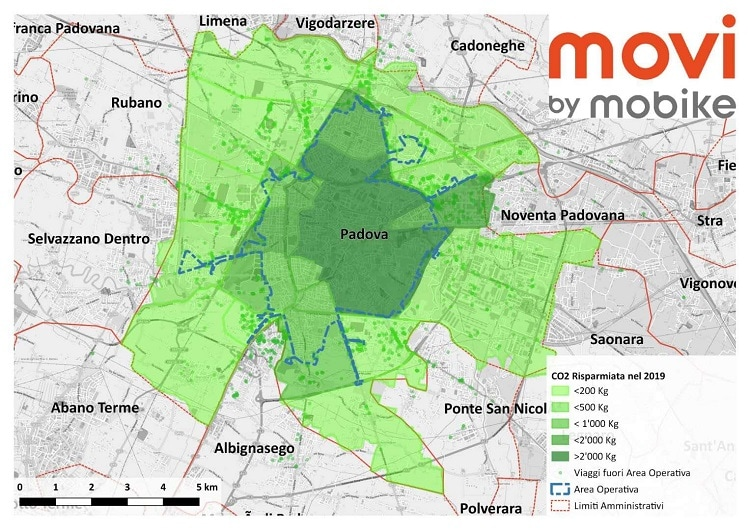
\includegraphics[width=8cm]{fig3.jpg}}
	\caption{Example of a figure caption.\cite{bibid}}
	\label{fig}
\end{figure}

\section{State of the art}
% \subsection{Abbreviations and Acronyms}\label{AA}
State of the art non solamente della letteratura ma anche di quello che viene offerto sul mercato

\section{Proposed solution}

	The idea is to show how this kind of devices can be portable enough to install on bikes
	companies like mobike could use them on their own bikes in order to gather data
	
	Dire che arduino è open source anche dal punto di vista hardware
	
	\subsection{The circuit}\label{AA}
		The circuit that composes this project is made of four main components:
		\begin{itemize}
			\item \textit{NodeMCU}: it's the hearts and brains of the device, this board is an open-source development kit based on the ESP8266 chip that allows for prototyping of IOT devices;
			\item \textit{MicroSD card reader}: 
			\item \textit{GPS sensor}: onboard led that indicates when it acquired the position
			\item \textit{MQ sensor}: as explained earlier the MQ sensor used in this project is MQ7 but it can easily be exchanged with other similar sensors that use the same board
		\end{itemize}
	
		It make detection by method of cycle high and low temperature, and detect CO when low temperature \cite{mq7}
	
		The other components are used for interacting with the user, as the leds and the button
		
		In the possible improvements section i explain how the circuit can be improved 
	
	\begin{figure}[htbp]
		\centerline{
\includegraphics[width=8cm]{fig1.png}}
		\caption{Example of a figure caption.}
		\label{fig}
	\end{figure}


\subsection{The Arduino software}
% \subsection{Abbreviations and Acronyms}\label{AA}
The reasons behind the choice of using Arduino's programming language instead of micropython \cite{micropyhton} because of the large community behind.

The arduino programming language is composed by a setup function and a loop function
in the setup i control 

in the loop i check

\subsection{The cloud}
% \subsection{Abbreviations and Acronyms}\label{AA}
Use of MQTT server 

snippet del json che arriva al server mqtt

\begin{lstlisting}[language=json,firstnumber=1]
{
    "id": "318",
    "air": "10.77",
    "lt": "45.39658",
    "lg": "11.88528",
    "dt": "260220.12283200",
    "tpc": "cocco"
}
\end{lstlisting}

\subsection{Possible total cost}

	most of these parts are open source and can be found sold on 
	
\section{Results and data analysis}\label{AA}
	\subsection{Test scenarios}

		\subsubsection{Prototype test}

		\subsubsection{Real life implementation}
			% \subsection{Abbreviations and Acronyms}\label{AA}
			State of the art
	
	\begin{figure}[htbp]
		\centerline{\includegraphics[width=8cm]{fig2.png}}
		\caption{Example of a figure caption.}
		\label{fig}
	\end{figure}

\section{Future improvements}

	In this section 
	
	\subsection{Hardware improvements}
	
		There are various improvements that could be made to the circuit and the hardware used, for example in this project using one single air quality sensor could be seen as a drawback since we could take advantage of the cheapness of these sensors
		
		It is possible to add multiple sensors by expanding the analog inputs using an \textit{Analog to Digital Converter} (ADC)
		
		that converts an analog voltage on a pin to a digital number. By converting from the analog world to the digital world, we can begin to use electronics to interface to the analog world around us.\cite{adc}
	
		In case we would want to use another transmission medium instead of wifi we could think about switching boards and use an arduino leonardo or an arduino uno or whatever iteration possible
	
	\subsection{Software improvements}
	
		Supposed we use the same architecture we can improve the software such that instead of looking for the ap and snding the data only when the button is pressef it could be set such that 
		
	\subsection{Cloud services improvements}
	
		In the development of this project I was forced by the we server host altervista.org to connect to the database only from within
		
		connections within its domain
		
		i was not able to allow the lambda to insert the data directly in the database, so I was forced to create an intermediate webpage to insert that data
		
		for this reason a possible improvement could be 

\section{Conclusions and future work}
This paper describes the implementation of a wireless IoT system capable to gather data from air and send it to the cloud in order to be analyzed and displayed.

%\subsection{Units}
%\begin{itemize}
%\item Use either SI (MKS) or CGS as primary units. (SI units are encouraged.) English units may be used as secondary units (in parentheses). An exception would be the use of English units as identifiers in trade, such as ``3.5-inch disk drive''.
%\item Avoid combining SI and CGS units, such as current in amperes and magnetic field in oersteds. This often leads to confusion because equations do not balance dimensionally. If you must use mixed units, clearly state the units for each quantity that you use in an equation.
%\item Do not mix complete spellings and abbreviations of units: ``Wb/m\textsuperscript{2}'' or ``webers per square meter'', not ``webers/m\textsuperscript{2}''. Spell out units when they appear in text: ``. . . a few henries'', not ``. . . a few H''.
%\item Use a zero before decimal points: ``0.25'', not ``.25''. Use ``cm\textsuperscript{3}'', not ``cc''.)
%\end{itemize}
%
%\subsection{Equations}
%Number equations consecutively. To make your 
%equations more compact, you may use the solidus (~/~), the exp function, or 
%appropriate exponents. Italicize Roman symbols for quantities and variables, 
%but not Greek symbols. Use a long dash rather than a hyphen for a minus 
%sign. Punctuate equations with commas or periods when they are part of a 
%sentence, as in:
%\begin{equation}
%a+b=\gamma\label{eq}
%\end{equation}
%
%Be sure that the 
%symbols in your equation have been defined before or immediately following 
%the equation. Use ``\eqref{eq}'', not ``Eq.~\eqref{eq}'' or ``equation \eqref{eq}'', except at 
%the beginning of a sentence: ``Equation \eqref{eq} is . . .''
%
%\subsection{\LaTeX-Specific Advice}
%
%Please use ``soft'' (e.g., \verb|\eqref{Eq}|) cross references instead
%of ``hard'' references (e.g., \verb|(1)|). That will make it possible
%to combine sections, add equations, or change the order of ures or
%citations without having to go through the file line by line.
%
%Please don't use the \verb|{eqnarray}| equation environment. Use
%\verb|{align}| or \verb|{IEEEeqnarray}| instead. The \verb|{eqnarray}|
%environment leaves unsightly spaces around relation symbols.
%
%Please note that the \verb|{subequations}| environment in {\LaTeX}
%will increment the main equation counter even when there are no
%equation numbers displayed. If you forget that, you might write an
%article in which the equation numbers skip from (17) to (20), causing
%the copy editors to wonder if you've discovered a new method of
%counting.
%
%{\BibTeX} does not work by magic. It doesn't get the bibliographic
%data from thin air but from .bib files. If you use {\BibTeX} to produce a
%bibliography you must send the .bib files. 
%
%{\LaTeX} can't read your mind. If you assign the same label to a
%subsubsection and a table, you might find that Table I has been cross
%referenced as Table IV-B3. 
%
%{\LaTeX} does not have precognitive abilities. If you put a
%\verb|\label| command before the command that updates the counter it's
%supposed to be using, the label will pick up the last counter to be
%cross referenced instead. In particular, a \verb|\label| command
%should not go before the caption of a figure or a table.
%
%Do not use \verb|\nonumber| inside the \verb|{array}| environment. It
%will not stop equation numbers inside \verb|{array}| (there won't be
%any anyway) and it might stop a wanted equation number in the
%surrounding equation.
%
%\subsection{Some Common Mistakes}\label{SCM}
%\begin{itemize}
%\item The word ``data'' is plural, not singular.
%\item The subscript for the permeability of vacuum $\mu_{0}$, and other common scientific constants, is zero with subscript formatting, not a lowercase letter ``o''.
%\item In American English, commas, semicolons, periods, question and exclamation marks are located within quotation marks only when a complete thought or name is cited, such as a title or full quotation. When quotation marks are used, instead of a bold or italic typeface, to highlight a word or phrase, punctuation should appear outside of the quotation marks. A parenthetical phrase or statement at the end of a sentence is punctuated outside of the closing parenthesis (like this). (A parenthetical sentence is punctuated within the parentheses.)
%\item A graph within a graph is an ``inset'', not an ``insert''. The word alternatively is preferred to the word ``alternately'' (unless you really mean something that alternates).
%\item Do not use the word ``essentially'' to mean ``approximately'' or ``effectively''.
%\item In your paper title, if the words ``that uses'' can accurately replace the word ``using'', capitalize the ``u''; if not, keep using lower-cased.
%\item Be aware of the different meanings of the homophones ``affect'' and ``effect'', ``complement'' and ``compliment'', ``discreet'' and ``discrete'', ``principal'' and ``principle''.
%\item Do not confuse ``imply'' and ``infer''.
%\item The prefix ``non'' is not a word; it should be joined to the word it modifies, usually without a hyphen.
%\item There is no period after the ``et'' in the Latin abbreviation ``et al.''.
%\item The abbreviation ``i.e.'' means ``that is'', and the abbreviation ``e.g.'' means ``for example''.
%\end{itemize}
%An excellent style manual for science writers is \cite{b7}.
%
%\subsection{Authors and Affiliations}
%\textbf{The class file is designed for, but not limited to, six authors.} A 
%minimum of one author is required for all conference articles. Author names 
%should be listed starting from left to right and then moving down to the 
%next line. This is the author sequence that will be used in future citations 
%and by indexing services. Names should not be listed in columns nor group by 
%affiliation. Please keep your affiliations as succinct as possible (for 
%example, do not differentiate among departments of the same organization).
%
%\subsection{Identify the Headings}
%Headings, or heads, are organizational devices that guide the reader through 
%your paper. There are two types: component heads and text heads.
%
%Component heads identify the different components of your paper and are not 
%topically subordinate to each other. Examples include Acknowledgments and 
%References and, for these, the correct style to use is ``Heading 5''. Use 
%``figure caption'' for your Figure captions, and ``table head'' for your 
%table title. Run-in heads, such as ``Abstract'', will require you to apply a 
%style (in this case, italic) in addition to the style provided by the drop 
%down menu to differentiate the head from the text.
%
%Text heads organize the topics on a relational, hierarchical basis. For 
%example, the paper title is the primary text head because all subsequent 
%material relates and elaborates on this one topic. If there are two or more 
%sub-topics, the next level head (uppercase Roman numerals) should be used 
%and, conversely, if there are not at least two sub-topics, then no subheads 
%should be introduced.
%
%\subsection{Figures and Tables}
%\paragraph{Positioning Figures and Tables} Place figures and tables at the top and 
%bottom of columns. Avoid placing them in the middle of columns. Large 
%figures and tables may span across both columns. Figure captions should be 
%below the figures; table heads should appear above the tables. Insert 
%figures and tables after they are cited in the text. Use the abbreviation 
%``Fig.~\ref{fig}'', even at the beginning of a sentence.
%
%\begin{table}[htbp]
%\caption{Table Type Styles}
%\begin{center}
%\begin{tabular}{|c|c|c|c|}
%\hline
%\textbf{Table}&\multicolumn{3}{|c|}{\textbf{Table Column Head}} \\
%\cline{2-4} 
%\textbf{Head} & \textbf{\textit{Table column subhead}}& \textbf{\textit{Subhead}}& \textbf{\textit{Subhead}} \\
%\hline
%copy& More table copy$^{\mathrm{a}}$& &  \\
%\hline
%\multicolumn{4}{l}{$^{\mathrm{a}}$Sample of a Table footnote.}
%\end{tabular}
%\label{tab1}
%\end{center}
%\end{table}
%
%\begin{figure}[htbp]
%\centerline{
\includegraphics{fig1.png}}
%\caption{Example of a figure caption.}
%\label{fig}
%\end{figure}
%
%Figure Labels: Use 8 point Times New Roman for Figure labels. Use words 
%rather than symbols or abbreviations when writing Figure axis labels to 
%avoid confusing the reader. As an example, write the quantity 
%``Magnetization'', or ``Magnetization, M'', not just ``M''. If including 
%units in the label, present them within parentheses. Do not label axes only 
%with units. In the example, write ``Magnetization (A/m)'' or ``Magnetization 
%\{A[m(1)]\}'', not just ``A/m''. Do not label axes with a ratio of 
%quantities and units. For example, write ``Temperature (K)'', not 
%``Temperature/K''.

\section*{Acknowledgment}

The preferred spelling of the word ``acknowledgment'' in America is without 
an ``e'' after the ``g''. Avoid the stilted expression ``one of us (R. B. 
G.) thanks $\ldots$''. Instead, try ``R. B. G. thanks$\ldots$''. Put sponsor 
acknowledgments in the unnumbered footnote on the first page.

%\section*{References}
%
%Please number citations consecutively within brackets \cite{b1}. The 
%sentence punctuation follows the bracket \cite{b2}. Refer simply to the reference 
%number, as in \cite{b3}---do not use ``Ref. \cite{b3}'' or ``reference \cite{b3}'' except at 
%the beginning of a sentence: ``Reference \cite{b3} was the first $\ldots$''
%
%Number footnotes separately in superscripts. Place the actual footnote at 
%the bottom of the column in which it was cited. Do not put footnotes in the 
%abstract or reference list. Use letters for table footnotes.
%
%Unless there are six authors or more give all authors' names; do not use 
%``et al.''. Papers that have not been published, even if they have been 
%submitted for publication, should be cited as ``unpublished'' \cite{b4}. Papers 
%that have been accepted for publication should be cited as ``in press'' \cite{b5}. 
%Capitalize only the first word in a paper title, except for proper nouns and 
%element symbols.
%
%For papers published in translation journals, please give the English 
%citation first, followed by the original foreign-language citation \cite{b6}.

\begin{thebibliography}{00}
	
\bibitem{luxemburg} \url{https://www.mobiliteit.lu/en/tickets/free-transport/}\\

\bibitem{b01} \url{https://www.wired.com/story/vehicle-future-bike/}\\

\bibitem{b02}  \href{https://www.ilsole24ore.com/art/in-bicicletta-lavoro-milano-risparmiate-275-tonnellate-co2-ACYBZ1FB}{https://www.ilsole24ore.com/art/in-bicicletta-lavoro-milano-risparmiate-275-tonnellate-co2-ACYBZ1FB}\\

\bibitem{b03} Official Arduino website: \url{https://www.arduino.cc/}\\

\bibitem{b04} Official Raspberry Pi website: \url{https://www.raspberrypi.org/}\\
	
\bibitem{b01} Lua based interactive firmware for ESP8266, ESP8285 and ESP32 \url{https://github.com/nodemcu/nodemcu-firmware}

http://www.padovaoggi.it/attualita/dati-mobike-padova-10-ottobre-2019.html

\bibitem{mobike} «In arrivo anche a Padova le E-Bike a pedalata assistita»: l'annuncio di Mobike
„«In arrivo anche a Padova le E-Bike a pedalata assistita»: l'annuncio di Mobike:  \href{http://www.padovaoggi.it/attualita/mobike-e-bike-dati-padova-21-febbraio-2020.html}{http://www.padovaoggi.it/attualita/mobike-e-bike-dati-padova-21-febbraio-2020.html}

https://arduinojson.org/
	
\bibitem{b20} G. Eason, B. Noble, and I. N. Sneddon, ``On certain integrals of Lipschitz-Hankel type involving products of Bessel functions,'' Phil. Trans. Roy. Soc. London, vol. A247, pp. 529--551, April 1955.
%\bibitem{b2} J. Clerk Maxwell, A Treatise on Electricity and Magnetism, 3rd ed., vol. 2. Oxford: Clarendon, 1892, pp.68--73.
%\bibitem{b3} I. S. Jacobs and C. P. Bean, ``Fine particles, thin films and exchange anisotropy,'' in Magnetism, vol. III, G. T. Rado and H. Suhl, Eds. New York: Academic, 1963, pp. 271--350.
%\bibitem{b4} K. Elissa, ``Title of paper if known,'' unpublished.
%\bibitem{b5} R. Nicole, ``Title of paper with only first word capitalized,'' J. Name Stand. Abbrev., in press.
%\bibitem{b6} Y. Yorozu, M. Hirano, K. Oka, and Y. Tagawa, ``Electron spectroscopy studies on magneto-optical media and plastic substrate interface,'' IEEE Transl. J. Magn. Japan, vol. 2, pp. 740--741, August 1987 [Digests 9th Annual Conf. Magnetics Japan, p. 301, 1982].
%\bibitem{b7} M. Young, The Technical Writer's Handbook. Mill Valley, CA: University Science, 1989.
\end{thebibliography}


%\vspace{12pt}
%\color{red}
%IEEE conference templates contain guidance text for composing and formatting conference papers. Please ensure that all template text is removed from your conference paper prior to submission to the conference. Failure to remove the template text from your paper may result in your paper not being published.

\end{document}
